\documentclass[12pt,letterpaper]{article}
\usepackage[top=2cm, bottom=4.5cm, left=2.5cm, right=2.5cm]{geometry}
\usepackage{fancyhdr}
\usepackage{amsmath}
\usepackage{graphicx}
\usepackage{float}
\setlength{\parindent}{0.0in}
\setlength{\parskip}{0.05in}

\newcommand\course{CSE 417T}
\newcommand\hwnumber{4}                  % <-- homework number
\newcommand\Name{Isabelle Xu and Clayton Knittel}         


\pagestyle{fancyplain}
\headheight 35pt
\lhead{\Name}
\chead{\textbf{\Large Homework \hwnumber}}
\rhead{\course \\ \today}
\lfoot{}
\cfoot{}
\rfoot{\small\thepage}
\headsep 1.5em

\begin{document}

\section*{Problem 1}

\begin{description}
	\item (a) \& (b)

\begin{figure}[H]
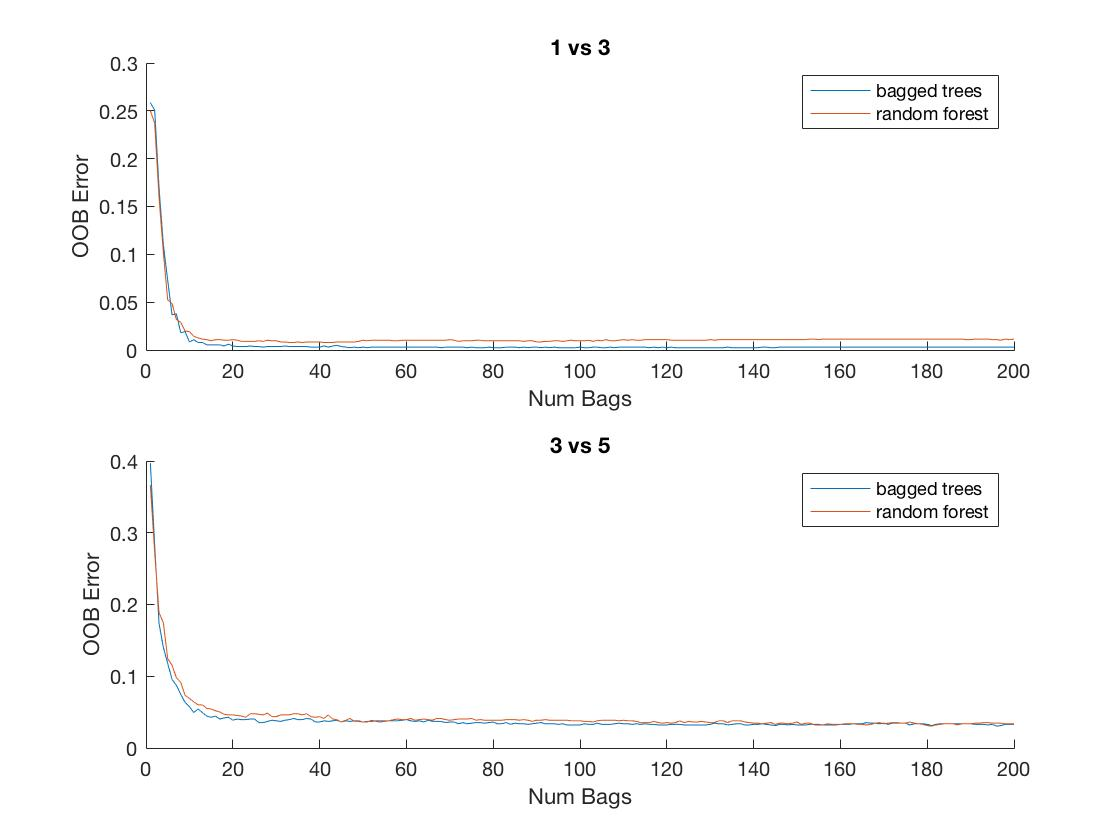
\includegraphics[scale=0.4]{image.jpg} \\\\
\end{figure}

	\item (c) 
\begin{table}[h]
\begin{tabular}{|l|l|l|l|}
\hline
\textbf{Decision Trees} & \multicolumn{2}{l|}{\textbf{Cross Val. Error}} & \textbf{Test Error} \\ \hline
1 vs 3                  & \multicolumn{2}{l|}{0.0090}                   & 0.0163             \\ \hline
3 vs 5                  & \multicolumn{2}{l|}{0.0659}                   & 0.1196	         \\ \hline
\end{tabular}
\end{table}
\begin{table}[h]
\begin{tabular}{|l|l|l|l|}
\hline
\textbf{200 Bagged Trees} & \multicolumn{2}{l|}{\textbf{OOB Error}} & \textbf{Test Error} \\ \hline
1 vs 3                    & \multicolumn{2}{l|}{0.0030}             & 0.0116              \\ \hline
3 vs 5                    & \multicolumn{2}{l|}{0.0338}             & 0.0890              \\ \hline
\end{tabular}
\end{table}
\begin{table}[h]
\begin{tabular}{|l|l|l|l|}
\hline
\textbf{Random Forest} & \multicolumn{2}{l|}{\textbf{OOB Error}} & \textbf{Test Error} \\ \hline
1 vs 3                    & \multicolumn{2}{l|}{0.0090}             & 0.0186              \\ \hline
3 vs 5                    & \multicolumn{2}{l|}{0.0371}             & 0.0767              \\ \hline
\end{tabular}
\end{table}
	\item (d) The results show that 200 bagged decision trees tend to perform better than a single decision tree in classification of digits in both the 1v3 and 3v5 data sets. Because each tree is only looking at some subset of the data, they all will tend to choose different features to differentiate by at each decision point, and thus each will be looking for different aspects of the data points at each step of the decision process when determining which digit it is most likely to be. Therefore, getting a majority vote among the trees is only likely if many different features of a number are like features of a three, not just a few particular ones. Random forests showed similar results to the bagged tree model as the algorithms for both are almost the same except for the use of split feature randomization, which in effect reduces the correlation between the bagged trees and therefore the out-of-sample error as the overfitting, which often results from high correlation in the normal bagged trees model, is addressed. Hence generally, it is expected for random forests to perform better.
	\\\\As for the differences between 1v3 and 3v5, both plots show very similar behavior except for the fact that 3v5 generally seemed more difficult to learn for all learning models due to how a 3 and a 5 have less distinguishing features between themselves. As a result all the different errors were higher for 3v5 than those of 1v3 all learning models. It's interesting to note that for 3v5 of random forest, the OOB error is slightly higher than that of bagged trees while its test error is lower than that of bagged trees in comparison to the results of 1v3 where both the OOB error and test error of random forest is larger than those of 200 bagged trees. 
	\\\\As we observed from our results, the effects of increasing the number of bags boiled down to a very steep decrease in OOB error before about 10 bags, which then it started to steadily decrease into a plateau around 30 bags. This could be attributed to the fact that OOB error should decease as the number of bags go up as we now probably have a fair sample of the data spread among the trees. For random forest, there is slightly more stochastic decision making on the algorithm's part (split feature randomization), so it takes longer for the error to settle. As a side note, introducing multiple bagged trees overall does reduce the variance, and by extension, the error rates since $E_out = bias + var$.

\end{description}
\section*{Problem 2}
\begin{description}
	\item (a) \& (b)
\begin{figure}[H]
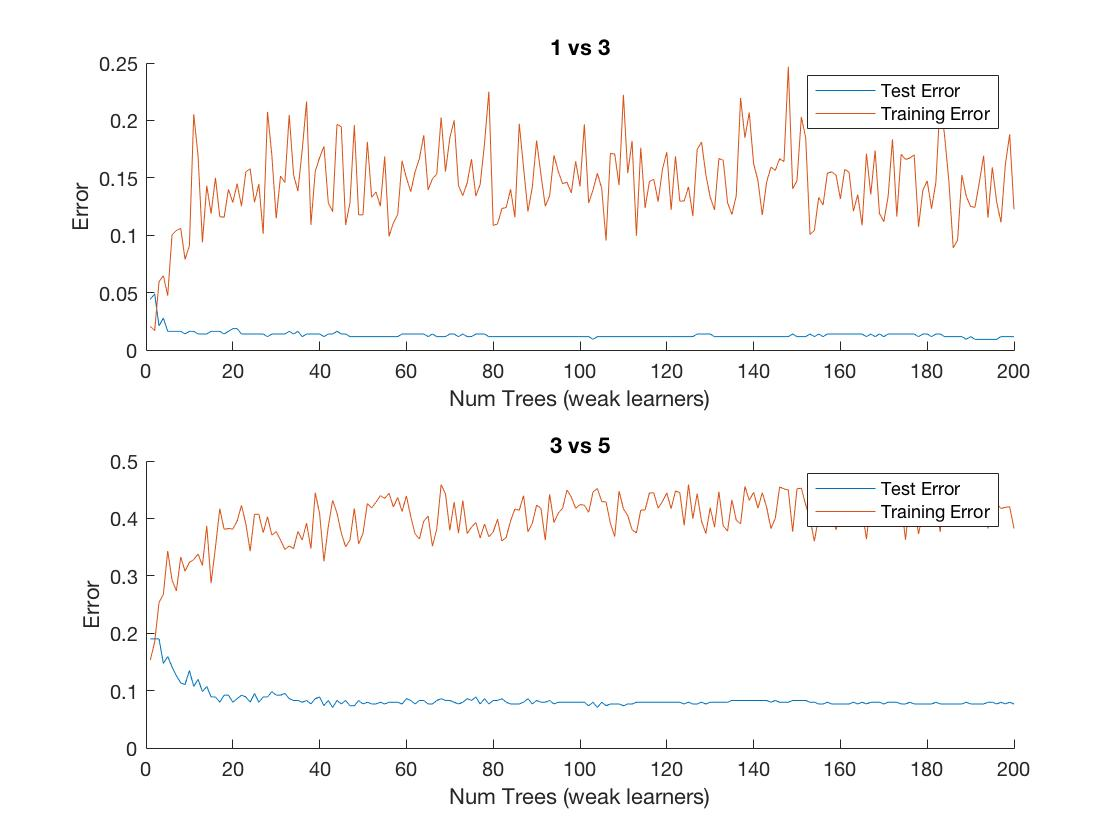
\includegraphics[scale=0.4]{image2.jpg} 
\end{figure}
\item (c) The differences between 1v3 and 3v5 for the adaboost model is that 1v3 resulted in lower test and training error by a scale of about 0.5.  This may also tie back to how 1v3 is considered easier to learn than 3v5 and therefore performing better. Specifically considering the adaboost algorithm, the training error for 3v5 appears to be on a steeper decline and this may be due to the fact that 3v5 was harder to learn, causing the algorithm to give more weight to inputs that are difficult to predict correctly and resulting in what we see in the plots. 
\\\\Tying into this we can see that as the number of weak learners increases, the training error for 1v3 appears to decreasing for later learners, hitting 0 before 10 learners. This could probably be attributed to how later learners in general have lower error as the upper bound for error decreases by a factor of 2 at each iteration because of $Z_t$ normalization. On the other hand for 3v5, as the number of weak learner increases, the training error takes a while to reach 0. Going back to how 3v5 is a more difficult problem, it is possible that adaboost had to account for noisier training data which in turn may have resulted in the increased weights of "problem" points and then the mislabeling of good samples, although the use of importance ($\alpha$) may have helped to alleviate this issue.
As for the generalization of adaboost as the number of weak learners increases, we can observe that it is quite good since the test error very rapidly goes down and appears to almost converge (plateau) before 20 weak learners. This could be due to the nature of using ensemble learning and aggregating the results of more and more weak learners, which naturally perform poorly by themselves, but much better when combined as they "boost" the accuracy of the learning model as bias is reduced. Hence we can expect $E_{out}$ to be low.

\end{description}

\section*{Problem 3}
\begin{description}
	\item (a) \& (b)
\begin{figure}[H]
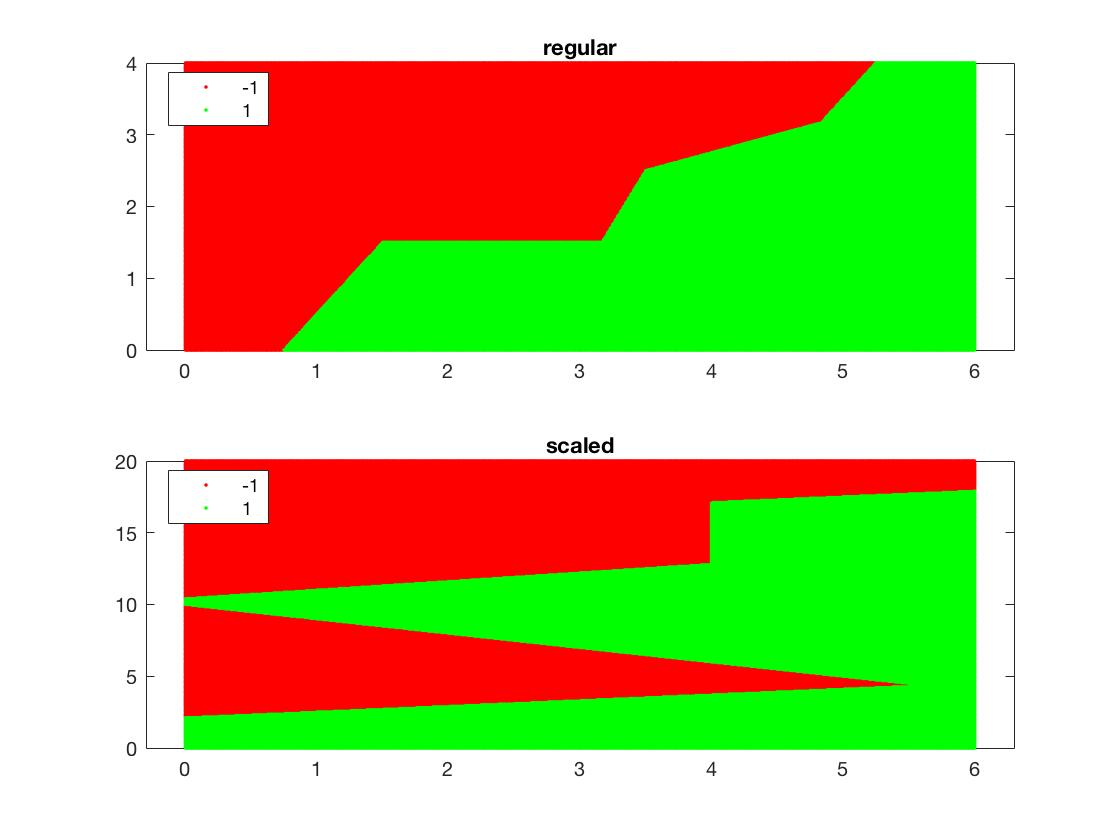
\includegraphics[scale=0.4]{image3.jpg} 
\end{figure}
	\item (c) Scaling the $x_2$ coordinate by 5 skewed the divide by a lot along the $x_1$ dimension. This put a lot more importance on the $x_1$ dimension of the coordinates, as points which were closer to a point, but separated mostly along the $x_2$ dimension, would get a lot farther away from that point after scaling $x_2$ by 5, but the $x_1$ coordinate remains unchanged. This caused the dividing line to become a lot sharper and “bend” a lot more to the data, which makes the predictor a lot more volatile to small changes in the input data. This is likely not a good effect.

\end{description}

\end{document}